\chapter{Introduction}
\section{Motivation}
Many applications require a fast, structured data store. Correctly implementing
a correct, performant custom solution in a general purpose programming language is a significant development cost.
Relational databases provide an attractive interface for describing the structure
and interactions with a store, but come with performance caveats and are not trivially integrated into applications.
\\
\\ For example a common OLTP pattern is to use a database to store the current state of a service.
\begin{figure}[h!]
    \centering
    
\includegraphics[scale=1]{introduction/_diagrams/slow_delta.pdf}
    \caption{A slow delta-database.}
\end{figure}
\noindent For many such applications the following holds.
\begin{enumerate}
    \setlength\itemsep{0em}
    \item Persistence requirements are weak enough to allow for in-memory only storage (optionally durability by replication).
    \item Each instance of the application is the sole interactor with the data store.
    \item Invariants/Constraints about the data must be maintained by the store.
    \item The schema and parameterized queries used are known at compile time. \label{lab:known_queries_item}
\end{enumerate}
Another more common pattern is to use implement complex state of an application in a general purpose programming language.

\begin{figure}[h!]
    \centering
    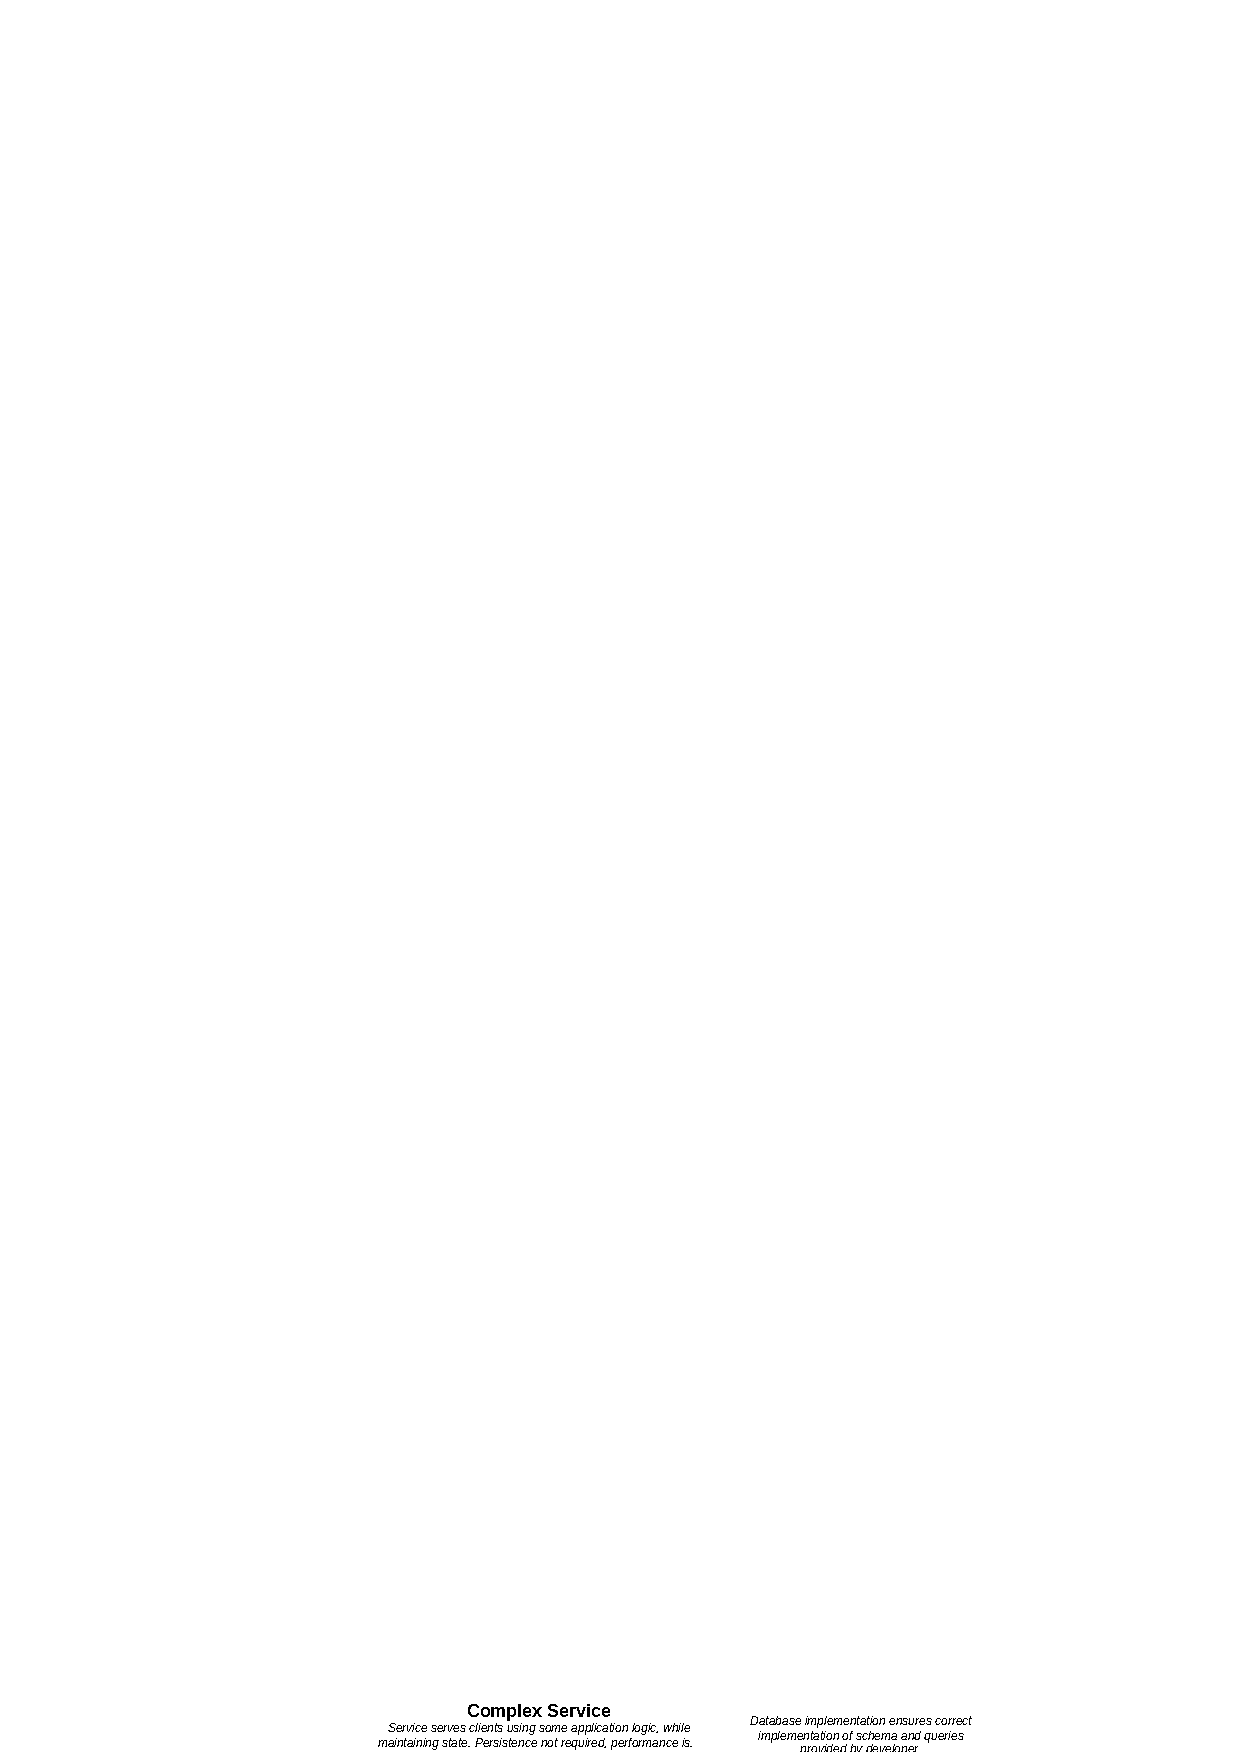
\includegraphics[scale=1]{introduction/_diagrams/complex_service.pdf}
    \caption{A typical complex service.}
\end{figure}

Much like the first pattern, a schema and set of queries including constraints are present. The
burden is either on the programmer to implement, or on the performance of the application when using the
convenience of a query language \& database.
\\
\\ A spectrum of solutions exist to embed a store in an application, here generally placed according to the strength of abstraction provided.
\begin{figure}[h!]
    \centering
    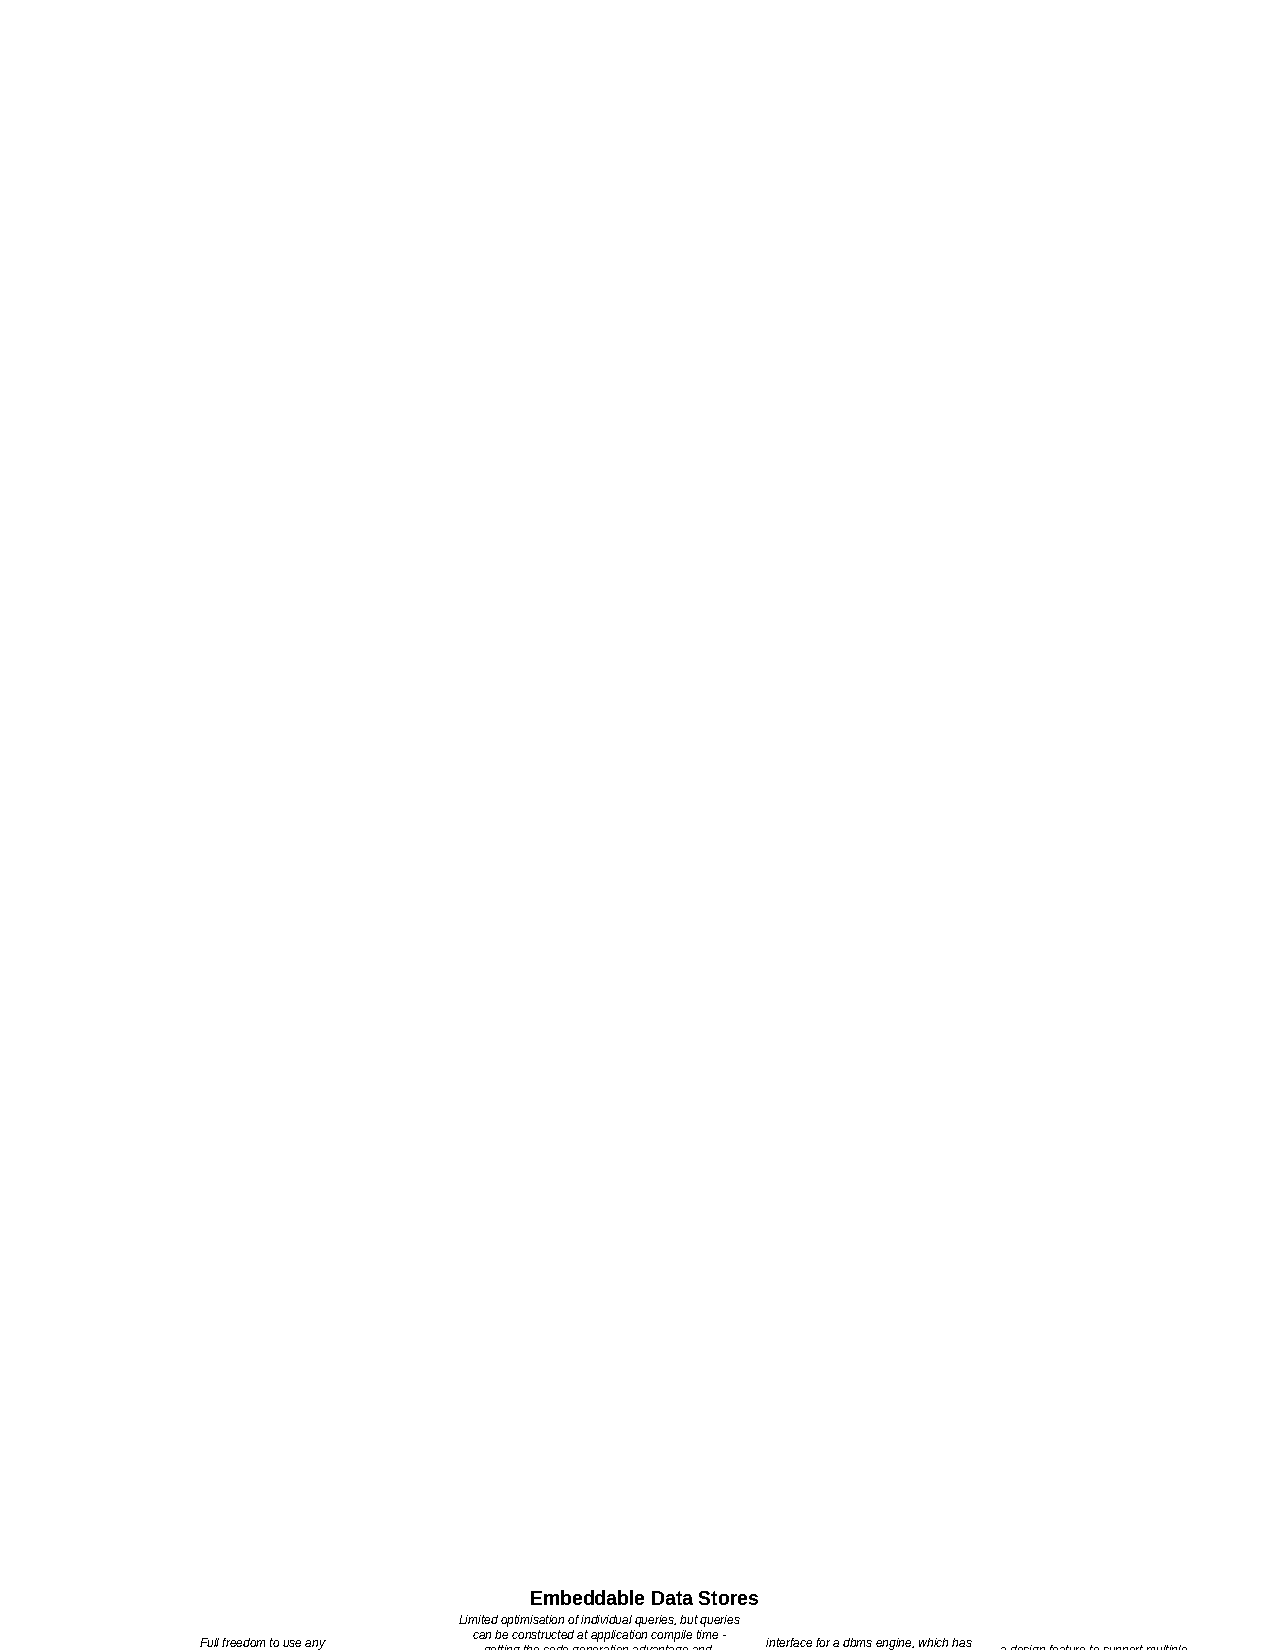
\includegraphics[width=\textwidth]{introduction/_diagrams/problem_space.pdf}
    \caption{A spectrum of data processing abstractions.}
\end{figure}
Unfortunately the strongest abstractions are present in embedded databases that do not take advantage of \ref{lab:known_queries_item} as by design
they both support schema changes, and are independent from the host language. For example duckDB is embeddable in Python, Java, Julia (and other)
applications. 
\\
\\The typical embedded database design is just an in-memory database, packaged to be in the same process an application.
\begin{figure}[h!]
    \centering
    \includegraphics[width=\textwidth]{introduction/_diagrams/typical_system.pdf}
    \caption{Typical Embedded Database System}
\end{figure}
\noindent An ideal system would allow such a datastore to be expressed in a query language, with an embeddable
implementation generated for use, and optimised using the full knowledge of the query set \& schema. It would also provide a strong compile time guarantee on the correctness of all queries.
\\
\\ No such ideal system exists, so we shall build it.

\section{Contributions}
\begin{center}
    \begin{tabular}{l p{.8\textwidth}}
        \textbf{emDB} & A schema-compiler demonstrating significant performance improvements over SQLite and DuckDB on a selection queries. \\
        \textbf{Combi} & A performant combinator library used for parsing rust tokenstreams, supporting multiple syntax errors without needing error node in the produced AST. \\
    \end{tabular}
\end{center}